\section{大学におけるソフトウェア開発実習の問題と問題に対する対処}

本節では,大学においてソフトウェア開発実習を行う際に考慮しなければならない問題について述べる.

考慮する必要がある点は大きく分けて以下の3点である.

\begin{itemize}
\item[・] アジャイルで求められるソフトウェア開発のスキル
\item[・] アジャイルにおける開発チームと受講生間のプログラミングのレベル差
\item[・] アジャイルのための環境
\end{itemize}

\subsection{アジャイルソフトウェア開発手法で求められるソフトウェア開発のスキル}

アジャイルを実践するには,前章で述べたようなことができる,または前節で述べたようなツールを使える必要がある.

つまり

\begin{itemize}
\item[・]問題点や要求を分析しソフトウェアの動作を変更できる
\item[・]ソフトウェアの変更点に対してのテストコードを書ける
\item[・]アプリケーションフレームワークを利用しプロダクトコードが書ける
\item[・]バージョン管理システムを利用してコードを管理できる
\item[・]継続的インテグレーションシステムを利用し,ソフトウェアの品質を保つことが出来る
\end{itemize}

以上が求められる.

しかし,上記のスキルはソフトウェア開発に置いて必要なことであり,コンピューターサイエンスとして必須では無いことから,これらのスキルを身につけるための授業が設置してあるとは考えづらい.(+だからRailsやGitやCIは本授業で取り扱う話を差し込む)アプリケーションフレームワークを利用することは,対象のプログラミング言語に対しての最低限の理解\footnote{例えば,クラスベースのオブジェクト指向プログラミングをサポートしているプログラミング言語ならば,クラスの記述方法や拡張方法,クラスから生成したインスタンスの利用方法などがあげられる}が必要となる.またWebアプリケーションのためのフレームワークならば,Web技術\footnote{Web技術とはHTMLやCSS,URLとプログラムの関係性やセッション,クッキーなどのこと}に対しての理解が必要となる.よって本研究で提案する授業はこれらの技術を習得もしくは理解していることを前提とする.


\subsection{受講生間のプログラミングのレベルの差}

アジャイルにおけるチームメンバーは,自立的かつ自己組織的なメンバーが求められる.大学での授業であるという問題を考えなければ,ソフトウェア開発実習でもチームを編成し授業を実施するのが良いだろう.
しかし,ソフトウェア開発実習を受講する学生のプログラミングのレベルの差があり,グループワークでの授業を実施すると,グループの間のプログラミングができる人とできない人の間に割り振られるタスクの量と質に差がでる.(+タスクをこなす量に差がでると,個々人が授業目標,授業目的を達成できない)タスクの割り振りによって,受講者が経験することが異なるのは避けたい.

この問題に対しては,授業の目標が「アジャイルに参加できるようになる」であることも考慮し,グループワーク形式の授業を採用せず,開発は参加者が各々に取り組む形を取ることで受講生間のレベル差の問題に対処する.

\subsection{アジャイルソフトウェア開発のための環境}

本来であれば,使用するツールや開発フローは出来る限り,企業が使用しているものに近づけたい.
しかし,環境の構築は知識を要求し,正しく動作するかの検証が必要なために手間がかかる.
本研究で提案する授業は,ソフトウェア開発に必要な手法やプログラミングを学ぶことであり環境を用意することではないので,サービスを利用する,ツールを用いる,学習の用途として不要な箇所は簡略化することで解決策を用意する必要がある.

(本文章に対しての理由を後ほど記述する)
開発環境の用意に関しては,予め利用する用意された仮想マシンのイメージを配布し,利用してもらうことで開発環境を用意する手間を省く.実行環境としてはHeroku\footnote{Webアプリケーションと呼ばれるソフトウェアを実行する際に管理する必要のある,Webサーバー,アプリケーションサーバー,RDBMS,DNSなど自分のプログラム以外のほぼ全てを管理してくれるサービス}というPaaS\footnote{Platform as a Service の略}を用いる.コードホスティングサーバーとして利用するサービスはGitHubを利用し,継続的インテグレーションツールとしてはCircleCIというSaaS\footnote{Software as a Serviceの略}を用いる.


\begin{figure}[H]
\centering
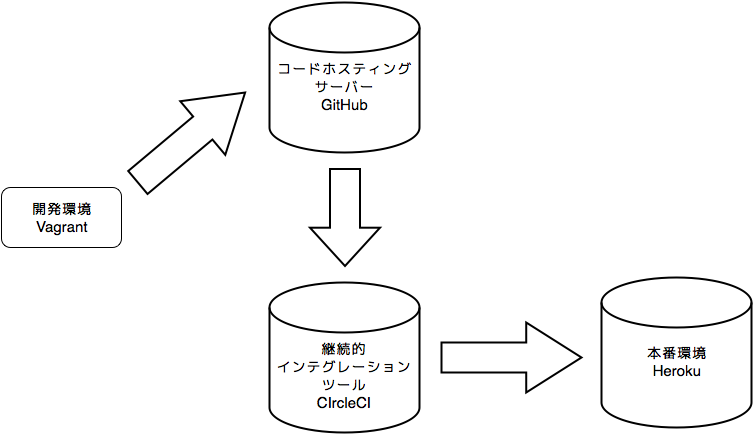
\includegraphics[height=8cm]{./assets/images/class_dev_env.png}
\caption{授業で用いる開発の環境概要図}
\label{fig:class_dev_env}
\end{figure}
